\documentclass[a4paper,14pt,russian]{extreport}
\usepackage[russian]{babel}

\usepackage{../common/dsturep_ru} % оформление по ДСТУ 3008-95
\usepackage{import}
\usepackage{standalone}
\usepackage{comment}
\usepackage{bbm}

\usepackage{tikz}
\usepackage{tikz-3dplot}
\usetikzlibrary{calc}
\usetikzlibrary{plotmarks}
\usepackage{pgfplots}

%\usepackage{scrextend}
\usepackage{changepage}
\usepackage{caption}
\usepackage{listings}
%\usepackage[title,titletoc]{appendix}
%\usepackage{appendix}
\usepackage{longtable}
%\usepackage{slashbox}
\usepackage{diagbox}
\usepackage{lscape}
\usepackage{algorithmic}
\usepackage{algorithm}

\def\male{male}
\def\female{female}

\bibliographystyle{../common/utf8gost780u}

\usepackage[square,numbers,sort&compress]{natbib}
\renewcommand{\bibnumfmt}[1]{#1.\hfill} % нумерация источников в самом списке — через точку

\def\passYear{2017}
\def\faculty{физико-технический институт}
\def\department{Кафедра информационной безопасности}
\def\departmentHead{Н. В. Грайворонский}
\def\kind{Дипломна робота}
\def\level{магістр}
\def\specialityCode{8.04030101}
\def\specialityTitle{Прикладная математика}
\def\theme{Решение нелинейных уравнений}
\def\gender{female}
\def\mentorGender{male}
\def\course{3}
\def\group{ФИ-41}
\def\name{Лавягина Ольга Алексеевна}
\def\mentorRank{}
\def\mentorName{Стёпочкина Ирина Валерьевна}
\def\reviewerRank{Rank}
\def\reviewerName{Name}
\def\subject{Методы вычислений}



\begin{document}

\import{1_title/}{title.tex}

\clearpage

\pagenumbering{gobble}
%\import{3_abstract/}{main.tex}

\pagestyle{empty}
\thispagestyle{empty}
\tableofcontents

\clearpage
\pagenumbering{arabic}
\pagestyle{fancy}
\setcounter{page}{2}

\clearpage

\chapter{Значение точной функции решения $y \left( x \right) $}

Уравнение имеет вид $y' = \left( 1 - x^2 \right) y + F \left( x \right) $.
Необходимо взять
$$h = 0.1, \,
  x \left( 0 \right) = 0.$$

Пусть решение известно и определяется $y = e^x$ (вариант 8).
Начальное значение $y \left( x \left( 0 \right) \right) = y \left( 0 \right) = e^0 = 1$.

Необходимо подставить решение в уравнение и определить в правой части $F \left( x \right) $.

Подставляем $e^x = \left( 1 - x^2 \right) e^x + F \left( x \right) $,
откуда $F \left( x \right) = e^x - e^x + x^2 e^x = x^2 e^x$.

Таким образом,
известный вид уравнения $y' = \left( 1 - x^2 \right) y + x^2 e^x$ и его точное решение,
с помощью численных методов дальше строим приближённое решение.

\chapter{Значения приближённого решения $y \left( x \right) $ в тех же точках,
        полученные обоими методами}

Используем формулы Рунге-Кутта четвёртого порядка.
Они имеют вид
$$y_{i + 1} =
  y_i + \frac{1}{6} \cdot \left( k_1 + 2k_2 + 2k_3 + k_4 \right),$$
где
$$ \begin{cases}
    k_1 = h \cdot f \left( x_i, y_i \right), \\
    k_2 = h \cdot f \left( x_i + \frac{1}{2} \cdot h, \, y_i + \frac{1}{2} \cdot k_1 \right), \\
    k_3 = h \cdot f \left( x_i + \frac{1}{2} \cdot h, \, y_i + \frac{1}{2} \cdot k_2 \right), \\
    k_4 = h \cdot f \left( x_i + h, y_i + k_3 \right),
  \end{cases}$$
где $f \left( x_i, y_i \right) = \left( 1 - x^2 \right) y + x^2 e^x$.

Приближённое решение методом Адамса-Башфорта находится по формуле
$$y_{k + 1} =
  y_k + \frac{h}{24} \left( 55f_k - 59f_{k - 1} + 37f_{k - 2} - 9f_{k - 3} \right).$$
Метод обеспечиваем четвёртый порядок точности.

\chapter{Графики точного решения и обоих приближённых}

Графики точного решения и обоих приближённых изображены на рисунке \ref{fig:solution}.

\begin{figure}[h!]
  \centering
  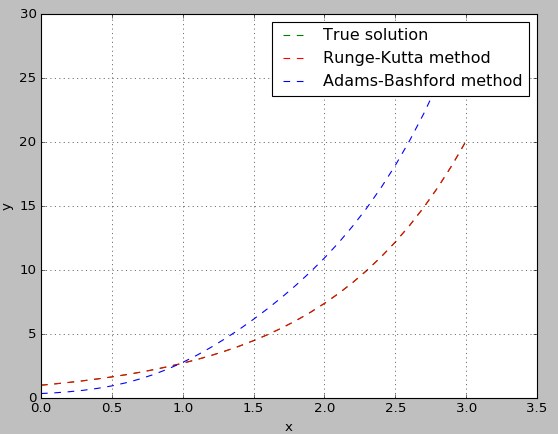
\includegraphics[width=.4\textwidth]{../code/solution.png}
  \caption{Графики точного решения и обоих приближённых}
  \label{fig:solution}
\end{figure}

Видно, что точное решение и решение методом Рунге-Кутта совпадают.

\chapter{Ошибки методов}

Для метода Рунге-Кутта была найдена теоретическая ошибка по формуле
$$e =
  \max \limits_i \frac{ \left| y_i^{ \left( h \right) } - y_{2i}^{ \frac{h}{2}} \right| }{15}.$$
Она равна $1.13914289957$.

Для обоих методов построены графики ошибок (рис. \ref{fig:error}),
найденных по формуле $ \left| trueSolution - methodSolution \right| $.

\begin{figure}[h!]
  \centering
  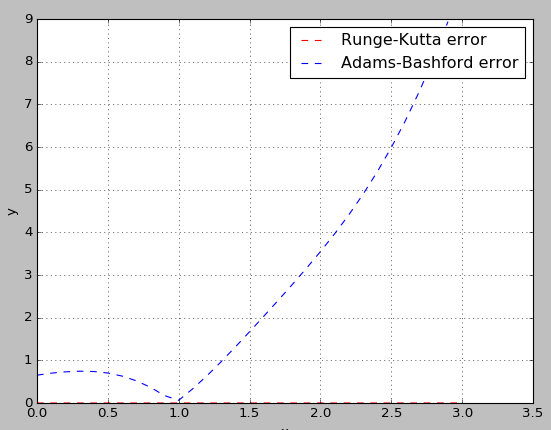
\includegraphics[width=.4\textwidth]{../code/error.png}
  \caption{Графики ошибок}
  \label{fig:error}
\end{figure}

\chapter{Листинг программы}

Листинг файла \_\_main\_\_.py
\lstset{inputencoding=utf8, extendedchars=\true}
\lstinputlisting[language=python,
                 basicstyle=\ttfamily\scriptsize]{../code/__main__.py}

 Листинг файла function.py
 \lstset{inputencoding=utf8, extendedchars=\true}
 \lstinputlisting[language=python,
                  basicstyle=\ttfamily\scriptsize]{../code/function.py}

Листинг файла runge\_kutta.py
\lstset{inputencoding=utf8, extendedchars=\true}
\lstinputlisting[language=python,
                 basicstyle=\ttfamily\scriptsize]{../code/runge_kutta.py}

 Листинг файла adams\_bashford.py
 \lstset{inputencoding=utf8, extendedchars=\true}
 \lstinputlisting[language=python,
                  basicstyle=\ttfamily\scriptsize]{../code/adams_bashford.py}

Листинг файла error.py
\lstset{inputencoding=utf8, extendedchars=\true}
\lstinputlisting[language=python,
                 basicstyle=\ttfamily\scriptsize]{../code/error.py}

\chapter*{Выводы}
\addcontentsline{toc}{chapter}{Выводы}

Было найдено решение уравнения вида $y' = f \left( x, y \right) $
с помощью методов Рунке-Кутта и Адамса-Батфорта.
Построены графики ошибок, из которых видно, что решение, полученное с помощью метода Рунке-Кутта,
совпадает с точным.

\end{document}
